\begin{task}
Доказать, используя поле экстремалей, что допустимая экстремаль в задаче

$$
\int_{t_{0}}^{t_{1}} \frac{\sqrt{1+\dot{x}^{2}}}{\sqrt{x}} d t \rightarrow \operatorname{extr}, \quad x\left(t_{0}\right)=x_{0}, \quad x\left(t_{1}\right)=x_{1}, \quad x>0
$$

является точкой глобального минимума (здесь $x_{0}>0, x_{1}>0$ ).

\textbf{Peшение.} Мы уже вычисляли экстремали в параметрическом виде:

$$
x=c(1-\cos \tau), \quad t-a=c(\tau-\sin \tau)
$$

где $a \in \mathbb{R}, c>0, \tau \in[0,2 \pi]$. Будем их обозначать $x(t, a, c)$.

Наша цель доказать: допустимая экстремаль будет точкой глобального минимума.

Сначала покажем, что $\dot{x}(t, a, c)$ строго убывает, при этом принимает все вещественные значения. В самом деле, $t(\tau)$ строго возрастает; $\frac{d x}{d t}=\frac{d x}{d \tau} \cdot \frac{d \tau}{d t}=\frac{\sin \tau}{1-\cos \tau} ;$ при $\tau \rightarrow+0$ предел равен $+\infty$, при $\tau \rightarrow 2 \pi-0$ предел $-\infty$. Производная по $\tau$ от $\frac{\sin \tau}{1-\cos \tau}$ равна $-\frac{1}{1-\cos \tau}<0$, так что $\ddot{x}<0$.

Утверждение. Для любых $t_{*}<t_{* *}, x_{*}>0, x_{* *}>0$ существуют единственные $c>0, a \in \mathbb{R}$ такие, что $x\left(t_{*}, a, c\right)=x_{*}, x\left(t_{* *}, a, c\right)=x_{* *}$, при этом $a$ и $c$ гладко зависят от $t_{*}, x_{*}, t_{* *}, x_{* *}$.

Доказательство. Пусть без ограничения общности $x_{*} \leq x_{* *}$.

Пусть $k=\frac{x_{* *}-x_{*}}{t_{* *}-t_{*}}, l$ - длина отрезка $\left[\left(t_{*}, x_{*}\right),\left(t_{* *}, x_{* *}\right)\right], \gamma=l / x_{*}$. Возьмем экстремаль $x(\cdot, 0,1)$ и покажем, что существуют такие $t^{\prime}<t^{\prime \prime}$, что $\frac{x\left(t^{\prime \prime}, 0,1\right)-x\left(t^{\prime}, 0,1\right)}{t^{\prime \prime}-t^{\prime}}=k$ и отношение длины отрезка $\left[\left(t^{\prime}, x\left(t^{\prime}, 0,1\right)\right),\left(t^{\prime \prime}, x\left(t^{\prime \prime}, 0,1\right)\right)\right]$ к $x\left(t^{\prime}, 0,1\right)$ равно $\gamma$; при этом $t^{\prime}$ и $t^{\prime \prime}$ определяются однозначно и гладко зависят от $k$ и $\gamma$.

\begin{figure}[h!]
    \centering
    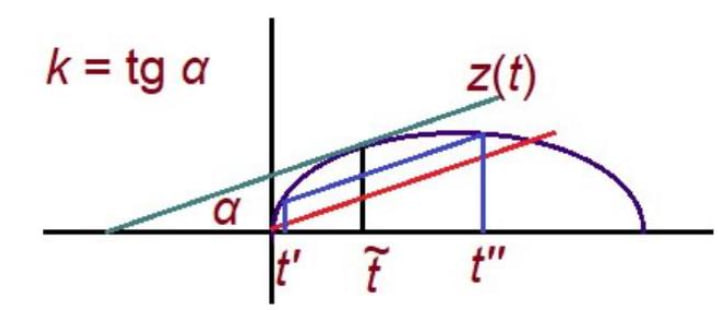
\includegraphics[width=0.99\linewidth]{tasks/task27/pic1.jpg}
\end{figure}

(Затем полагаем $c=x_{*} / x\left(t^{\prime}, 0,1\right), a=t_{*}-c t^{\prime}$ и получаем утверждение.)

Так как $\dot{x}(t, 0,1)$ строго убывает по $t$ и принимает все вещественные значения, то существует единственное $\tilde{t}$ такое, что $z(t)=x(\tilde{t}, 0,1)+k(t-\tilde{t})$ - касательная. Далее рассматриваем уравнение $x(t, 0,1)=z(t)-r$, где $r>0$. Так как вторая производная $x$ строго отрицательна, то количество корней не более 2 . Если решений ровно 2 , то получаем хорду $\left[\left(t_{r}^{\prime}, x_{r}^{\prime}\right),\left(t_{r}^{\prime \prime}, x_{r}^{\prime \prime}\right)\right]$ (ее концы - точки пересечения циклоиды и графика $z(t)-r$ ). При этом $t_{r}^{\prime}$ гладко зависит от $r$ (по теореме о неявной функции) и строго убывает по $r$ (а значит, и $x_{r}^{\prime}$ ), длина хорды $l_{r}$ строго возрастает по $r$; $x_{r}^{\prime}$ меняется от $x(\tilde{t}, 0,1)$ до 0 , а $l_{r}$ - от 0 до некоторого положительного числа. Значит, $l_{r} / x_{r}^{\prime}$ строго возрастает от 0 до $+\infty$ и при некотором $r>0$ равно $\gamma$ (это число $r$ единственно и гладко зависит от $\gamma$ ). Тем самым найдены $t^{\prime}$ и $t^{\prime \prime} . \diamond$

Докажем, что экстремаль в задаче о брахистохроне (с положительными $x_{0}, x_{1}$ ) будет точкой глобального минимума, используя поле экстремалей.

Пусть $t_{*}<t_{0}$ (достаточно близко к $t_{0}$, так, чтобы экстремаль гладко продолжалась в эту точку). Пусть $\hat{x}\left(t_{*}\right)=x_{*}>0$. Рассмотрим множество всех циклоид $x(t, b)$, проходящих через $\left(t_{*}, x_{*}\right)$; в качестве параметра $b$ можно взять $\dot{x}\left(t_{*}, b\right)=b$.

Пусть $\delta>0$ - достаточно малое число, $t_{*}<\tau<t_{1}+\delta, \xi>0$. В силу доказанного утверждения, существует (единственная) циклоида, проходящая через ( $t_{*}, x_{*}$ ) и $(\tau, \xi)$, при этом параметры, ее определяющие, гладко зависят от $\tau$, $\xi$. Значит, $b(\tau, \xi)$ - гладкая функция. Поэтому построенное семейство экстремалей образует центральное поле.

Наконец, $L_{\dot{x} \dot{x}}>0$, т.е. $L$ выпукла по $\dot{x}$. Поэтому по достаточному условию экстремаль будет точкой глобального минимума.
\end{task}